The \glspl{lut} are designed using the \gls{ib} method\cite{tishby2000information}. The \gls{ib} framework clusters an observed quantity $y$ into its compressed form $t$ such that $\max_{p(t|y)}I(X;T)$. The random variable $X=x$ is the designated quantity of primary relevance, e.g., a bit value, while the random variable $T=t\in\mathcal{T}=\{ 0,1,\dots, |\mathcal{T}|-1\}$ is the compressed or quantized observation. The deterministic mapping $p(t|y)$ can be treated as a \gls{lut} with $y$ and $t$ as input and output, respectively. 

Each message $t$ is associated with a \gls{lut} $L_x(t)$ which can be computed from the distribution $p(x,t)$ that is provided by the \gls{ib} solution.
Further, the finite alphabet $\mathcal{T}$ for the quantized messages is chosen such that 
\begin{align*}
L_{x}\left(t = \sfrac{|\mathcal{T}|}{2} - 1 - j\right)= - L_{x}\left(t = \sfrac{|\mathcal{T}|}{2} + j\right),
\end{align*}
where $ j=0, \cdots , \frac{|\mathcal{T}|}{2} - 1$. 
Moreover, $L_x(t)>L_x(t^\prime)$ if $t>t^\prime$, $\forall \: t,t^\prime \in \mathcal{T}$. Such a cluster assignment enables hard decisions of the bit $x$ as the first half of the alphabet translates to negative LLRs while the second half translates to positive LLRs.

\begin{figure}
    \centering
    \resizebox{0.5\columnwidth}{!}{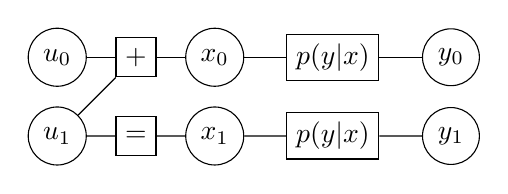
\begin{tikzpicture}[yscale=0.4, xscale=1, node distance=0.3cm, auto]
	
		\def \nodesize {0.5} %in cm
		\def \VertDist {2.5}
		\def \HorDist {1}
		\def \HorDisplace {0.5}
		
		\node (U0) at (0-\HorDist,0) [draw, circle, minimum width = \nodesize cm]{$u_0$};
		\node (U1) at (0-\HorDist,0-\VertDist) [draw, circle, minimum width = \nodesize cm]{$u_1$};%[align=center]{$U_1$};
		\node (Cn0) at (0,0) [draw, rectangle, minimum width = \nodesize cm,minimum height = \nodesize cm]{$+$};
		\node (Cn1) at (0,0-\VertDist) [draw, rectangle, minimum width = \nodesize cm,minimum height = \nodesize cm]{$=$};	
		\node (X0) at (\HorDist,0) [draw, circle, minimum width = \nodesize cm]{$x_0$};
		\node (X1) at (\HorDist,0-\VertDist) [draw, circle, minimum width = \nodesize cm]{$x_1$};
		\node (Cn2) at (2*\HorDist +\HorDisplace,0) [draw, rectangle, minimum width = \nodesize cm,minimum height = \nodesize cm]{$p(y|x)$};
		\node (Cn3) at (2*\HorDist +\HorDisplace,0-\VertDist) [draw, rectangle, minimum width = \nodesize cm,minimum height = \nodesize cm]{$p(y|x)$};	
		\node (Y0) at (3*\HorDist +2*\HorDisplace,0) [draw, circle, minimum width = \nodesize cm]{$y_0$};
		\node (Y1) at (3*\HorDist +2*\HorDisplace,0-\VertDist) [draw, circle, minimum width = \nodesize cm]{$y_1$};
		
		
		%[draw,circle,cross,minimum width=0.5 cm]
		\draw[-] (U0) -- (Cn0);
		\draw[-] (U1) -- (Cn1);
		\draw[-] (Cn0) -- (X0);
		\draw[-] (Cn1) -- (X1);
		\draw[-] (U1) -- (Cn0);
		\draw[-] (X0) -- (Cn2) --(Y0);
		\draw[-] (X1) -- (Cn3) --(Y1);
		
%		\node[draw,dashed,fit=(U0) (X1)] {};
		%\node[draw,dotted,color = darkred, fit=(U0) (X1),line width=1.0pt,line cap=round, dash pattern=on 0pt off 2\pgflinewidth] (block) {};
	
	\end{tikzpicture}}
    \caption{Setup for generating decoding \glspl{lut} on a single building block}
    \label{fig:N2_LUT_setup}
\end{figure}

\autoref{fig:N2_LUT_setup} is used to illustrate the process of generating decoding \glspl{lut} for a polar code of length $N=2$.  In the figure, the uncoded bits $\mvec{u}$ are transformed into coded bits $\mvec{x}$ and received as $\mvec{y}$ after transmission through a  quantized \gls{awgn} channel with transition probabilities $p(y|x)$.  The \gls{awgn} channel quantizer is designed for a certain noise variance $\sigma_N^2$ using the \gls{ib} method with $y \in \mathcal{T}$.

With the quantized channel outputs $[y_0,y_1]$ at hand, the \glspl{lut} for decoding $u_0$ and $u_1$ are generated by quantizing their bit channels  using the \gls{ib} method. For decoding $u_0$, the output $\mvec{y_0}=[y_0,y_1]$ of its bit channel are quantized into $t_0\in\mathcal{T}$ such that $\max_{p(t_0|\mvec{y}_0)}I(U_0;T_0)$. The deterministic mapping $p(t_0|\mvec{y}_0)$ can serve as a \gls{lut} that replaces the $f$ function. It maps $\mvec{y_0}$ to $t_0$ which, in turn, can be used to decode $u_0$ as 
\begin{align}\label{eqn:ib:estu}
\hat{u}_i = \begin{cases}
0\text{,} & \text{when } t_i >\sfrac{|\mathcal{T}|}{2}\\
1\text{,} & \text{otherwise.}
\end{cases}
\end{align}
with $i = 0$. 
Similarly, the output $\mvec{y_1}=[y_0,y_1,u_0]$ of the bit channel of $u_1$ is compressed to $t_1 \in \mathcal{T}$   aiming $\max_{p(t_1|\mvec{y}_1)}I(U_1;T_1)$. The \gls{lut} $p(t_1|\mvec{y}_1)$ can then replace the $g$ function, where it is used to map $\mvec{y}_1$ to $t_1$ and decode $u_1$ using \eqref{eqn:ib:estu}. 

For a polar code of length $N > 2$, the decoding \glspl{lut} are obtained by integrating the aforementioned mutual information preserving quantization into its density evolution\cite{shah_coarsely_2019}. These decoding \glspl{lut} then replace \eqref{eqn:sc:f} and \eqref{eqn:sc:g} in the \gls{sc} decoding.
This is illustrated for the root node in the decoder tree of Fig.\,\ref{fig:sc-tree}, and \glspl{lut} $p(t_0|\mvec{y}_0)$ and $p(t_1|\mvec{y}_1)$ obtained in this section. In this case, the \gls{llr} carrying vectors $\mvec{\alpha}$ get replaced with vectors of integer valued messages $\mvec{t}$. With $N_v{=}8$, $\mvec{t}_v$ will carry the  quantized channel outputs $y_0,\dots,y_7$. The \gls{lut} $p(t_i| y_i,y_{i + \sfrac{N_v}{2}})$, i.e., the mapping $p(t_0|\mvec{y}_0)$ with labels adjusted for $N{=}8$, will be used to generate the updates $\mvec{t}_l$ for the left child of the root node. Similarly, the updates $\mvec{t}_r$ for the right child will be generated using the \gls{lut}  $p(t_i| y_i,y_{i + \sfrac{N_v}{2}},\beta_l[i])$, i.e., the mapping $p(t_1|\mvec{y}_1)$ with adjusted labels. Note that  a separate decoding \gls{lut} is used for each edge in the \gls{sc} decoding tree, i.e, $2N{-}N$ \glspl{lut} in total. At the leaf nodes, \eqref{eqn:ib:estu} can be used to estimate $\bm{\hat{u}}$ from $t_l$ and $t_r$.  The decoder that uses the \glspl{lut} designed using the \gls{ib} framework is henceforth referred to as the \gls{ib} decoder.



\subsection{Hardware-Efficient Look-up Tables}\label{sec:lut:variants}

The  \glspl{lut} in Section \ref{sec:gen:lut} are obtained from quantized density evolution of a polar code. 
Thus the $N{-}1$ distinct $f$-operation \glspl{lut} are designed according to the check-node update rule, i.e., the so-called box-plus operation. 
The $g$ \glspl{lut} are designed according to the variable-node update rule.
From a hardware point of view, efficient implementation of one, e.g., $f$, \gls{lut} might not be valid for a different $f$ \gls{lut} because the two will have different truth tables. However, it is beneficial to reduce the number of distinct \glspl{lut} so that the same hardware-efficient realization can be used for multiple \glspl{lut}.

In \cite{shah_MSIB_2023}, \gls{lut}-based polar decoders were constructed where the min-sum approximation is utilized for designing the $f$ \glspl{lut} while, like \cite{shah_coarsely_2019}, the $g$ \glspl{lut} are designed using the \gls{ib} method. It was shown in \cite{shah_MSIB_2023} that the effect of using the approximate min-sum rule for \gls{lut} design on the error-correction performance of the decoder is negligible. Such a decoder is referred to as an \emph{MS-IB} decoder.  

In an MS-IB decoder, all the $f$ \glspl{lut} have the same input/output relation. The number of distinct  $f$ \glspl{lut}, w.r.t. an \gls{ib} decoder, thus reduces from $N-1$ to 1. Most importantly, the min-sum based $f$ \gls{lut} can be realized as a min-sum of the integer valued message $t_a,t_b \in \mathcal{T}$. 
Recall (cf. Section \ref{sec:gen:lut}) that the integer messages embed \gls{llr} information. The \gls{msb} of the \gls{lut} inputs can be treated as the sign of the associated \gls{llr} with $\text{\gls{msb}}=0$ meaning negative \gls{llr} and vice versa. The remaining bits can be seen as the input-message magnitude associated to the \gls{llr}. The min-sum operation of the input integer messages can be expressed as:
\begin{align}\label{eqn:lut:minsum}
    t_o = f( t_a - \Delta, t_b - \Delta) + \Delta, 
\end{align}
where $\Delta= \frac{|\mathcal{T}|-1}{2}$, $t_o \in \mathcal{T}$ and $f(\cdot,\cdot)$ is computed using \eqref{eqn:sc:f}.

In comparison to \eqref{eqn:sc:f}, the argument $\Delta$ in \eqref{eqn:lut:minsum} is used for pre- and post-processing of the min-sum operation. 
From an implementation viewpoint, this is equivalent to inverting the magnitude carrying bits of any input message as well as the output message, if it falls in the first half of the finite alphabet $\mathcal{T}$. This extra logic can be discarded if a partially flipped finite alphabet is used. 
More precisely, all the integer messages are relabeled such that they belong to the \emph{relabeled} finite alphabet $\mathcal{T}_{re} = \{3,2,1,0,4,5,6,7 \}$ instead of  $\mathcal{T} = \{0,1,2,3,4,5,6,7 \}$ for $|\mathcal{T}|=8$.
Under the relabeled alphabet, the min-sum expression of \eqref{eqn:sc:f} can directly be applied to integer-valued messages $t_a^\prime,t_b^\prime\in\mathcal{T}_{re}$. A \gls{lut}-based MS-IB decoder that  uses $\mathcal{T}_{re}$ is referred to as \emph{re-MS-IB} decoder. Relabeling has no effect on error-correction performance.


